\graphicspath{ {Figures/blood_donation/} }

\chapter{Εθελοντική αιμοδοσία}\label{ch:Βlood Donations}

\section{Εθελοντική αιμοδοσία}
	Στο παρόν κεφάλαιο αναλύουμε τις βασικές έννοιες σχετικά με την αιμοδοσία, οι οποίες εμπλέκονται στο θέμα της παρούσας διπλωματικής εργασίας.
	\subsection{Το αίμα}
	Το αίμα είναι το σπουδαιότερο βιολογικό υγρό του ανθρώπινου οργανισμού και αποτελεί ένα ανεκτίμητο προϊόν ζωής, το οποίο δεν μπορεί να κατασκευαστεί με συνθετικό τρόπο. Χωρίς την επαρκή ποσότητα αίματος, τα κύτταρα του ανθρώπινου σώματος δεν μπορούν να λάβουν το οξυγόνο και τα θρεπτικά συστατικά που τους είναι απαραίτητα για να επιβιώσουν \cite{aboutBlood}. Επιπλέον το σώμα δεν θα μπορούσε να αντιμετωπίσει βλαπτικούς παράγοντες, να αποβάλει τοξικά προϊόντα και να ρυθμίσει τις παραμέτρους του εσωτερικού του περιβάλλοντος \cite{circulatorySystem}. Αν και η τεράστια αξία και χρησιμότητα του αίματος είναι αδιαμφισβήτητη, η μη ύπαρξη αρκετών εθελοντικών αιμοδοσιών για να καλυφθούν οι ανάγκες για αίμα αποτελεί μείζων πρόβλημα.
	
	Το αίμα αποτελείται από ερυθρά αιμοσφαίρια, λευκά αιμοσφαίρια, αιμοπετάλια -τα οποία εναιωρούνται μέσα στο πλάσμα- και πρωτεΐνες. Στο σχήμα \ref{fig:basic_blood_diagram}  παρακάτω παρουσιάζονται τα διάφορα συστατικά από τα οποία αποτελείται το αίμα:
	\begin{figure}[h]
	    \centering
	    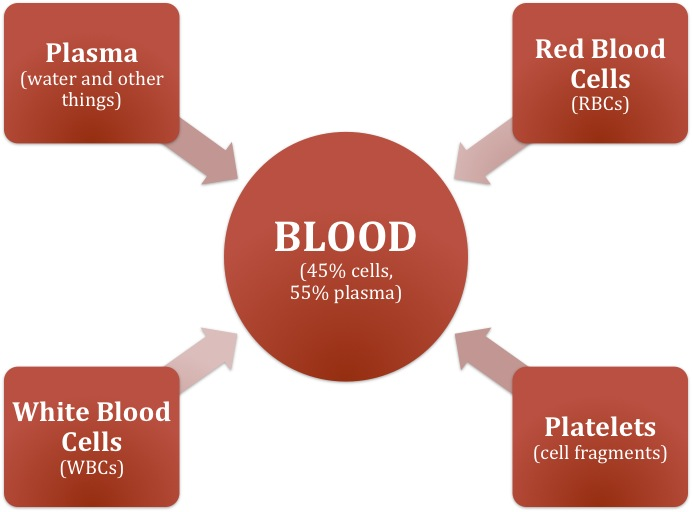
\includegraphics[width=0.7\textwidth]{basic_blood_diagram.jpg}
	    \caption{Συστατικά του αίματος}
	    \label{fig:basic_blood_diagram}
	\end{figure}
	 
	Το πλάσμα αποτελεί το μεγαλύτερο και κυριότερο συστατικό του αίματος, καταλαμβάνοντας το 55\% του συνολικού όγκου του. Είναι ένα υποκίτρινο υγρό μέσω του οποίου μεταφέρονται αιμοσφαίρια, πρωτεΐνες και άλλες ουσίες. Αποτελείται κατά 91,5\% από νερό, κατά 7\% από πρωτεΐνες, όπως η λευκωματίνη (αλβουμίνη), οι σφαιρίνες και το ινωδογόνο, και κατά 1,5\% από άλλες ουσίες, όπως θρεπτικά συστατικά, ορμόνες, αναπνευστικά αέρια, ηλεκτρολύτες, βιταμίνες και άχρηστες αζωτούχες ουσίες \cite{bloodPlasma}. Η κύρια λειτουργία που επιτελεί είναι η μεταφορά υγρών και υδατοδιάλυτων ουσιών, όπως είναι οι ορμόνες.

	Το υπόλοιπο 45\% του αίματος αποτελείται από ερυθρά αιμοσφαίρια, λευκά αιμοσφαίρια και αιμοπετάλια. Τα ερυθρά αιμοσφαίρια είναι τα πιο πολυάριθμα κύτταρα σε κυκλοφορία και δίνουν στο αίμα το χαρακτηριστικό κόκκινο χρώμα του. Τα ερυθρά αιμοσφαίρια χρησιμοποιούνται ευρέως, για να αναπληρώνουν την απώλεια αίματος που προκαλείται από αιμορραγία κατά τη γέννα, κατά τη διάρκεια χειρουργικής επέμβασης και κατά τη διάρκεια ατυχημάτων. Η μετάγγιση ερυθρών αιμοσφαιρίων μπορεί επίσης να είναι σωτήρια για τη ζωή του ασθενούς σε συγκεκριμένους τύπους αναιμίας. Η λειτουργία τους αφορά τη διατήρηση των ιστών στη ζωή καθώς μεταφέρουν σε αυτούς οξυγόνο και απομακρύνουν το διοξείδιο του άνθρακα. Η εκατοστιαία αναλογία ερυθρών αιμοσφαιρίων ανά μονάδα όγκου αίματος ονομάζεται αιματοκρίτης \cite{hematologyBasics}.
	
	Τα λευκά αιμοσφαίρια ή λευκοκύτταρα (WBC) αποτελούν λιγότερο από το 1\% του ολικού αίματος. Η πρωταρχική λειτουργία των λευκοκυττάρων είναι η καταπολέμηση των λοιμώξεων μέσω της επίθεσης και της καταστροφής επιβλαβών ξένων ουσιών. Σχηματίζονται στον μυελό των οστών, στον σπλήνα και στους λεμφαδένες \cite{whiteBloodCells}.
	
	Τα αιμοπετάλια ή θρομβοκύτταρα παράγονται από τον μυελό των οστών και αποτελούν λιγότερο από το 1\% του πλήρους αίματος. Παίζουν καθοριστικό ρόλο στην πήξη του αίματος και την αιμόσταση, δηλαδή στην αναστολή της αιμορραγίας ή της κυκλοφορίας. Σχηματίζουν θρόμβους ώστε να αποτρέπεται η διαρροή αίματος από τις πληγές και αν ο αριθμός τους είναι χαμηλός, αυτό μπορεί να οδηγήσει σε εύκολη δημιουργία μωλώπων και σε μεγάλη αιμορραγία. Οι ασθενείς που έχουν λευχαιμία ή ανεπάρκεια του μυελού των οστών, συνήθως έχουν χαμηλό ποσοστό αιμοπεταλίων με αποτέλεσμα να χρειάζονται αιμοπετάλια, για να διαφυλάξουν τη λειτουργία της πήξης του αίματός τους \cite{hematologyBasics}.
	
	Στο σχήμα \ref{fig:blood_cells_characteristics} βλέπουμε μια σύνοψη των βασικών χαρακτηριστικών των συστατικών του αίματος.
\begin{figure}[H]
	    \centering
	    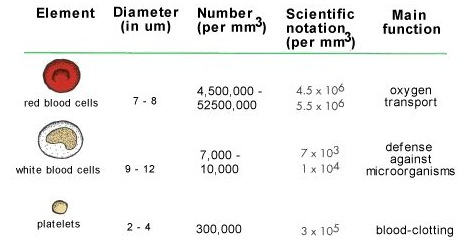
\includegraphics[width=0.7\textwidth]{blood_cells_characteristics.jpg}
	    \caption{Χαρακτηριστικά των κυττάρων του αίματος}
	    \label{fig:blood_cells_characteristics}
\end{figure}

	Τα κύτταρα του αίματος ανανεώνονται συνεχώς, όπως φαίνεται από τη διάρκεια ζωής στο αίμα των ερυθρών αιμοσφαιρίων (120 ημέρες), των αιμοπεταλίων (10 ημέρες) και των κοκκιοκυττάρων (9 ώρες). Ο χρόνος ζωής των λεμφοκυττάρων (Τ και Β κυττάρων) ποικίλλει εξαιρετικά από ώρες έως χρόνια. Η παραγωγή ενεργών κυττάρων του αίματος λαμβάνει χώρα κατά κύριο λόγο στον μυελό των οστών. Ωστόσο ο σπλήνας, οι λεμφαδένες και οι βοηθητικοί λεμφοειδείς ιστοί είναι επίσης θέσεις συνεχιζόμενης παραγωγής κυττάρων, κυρίως λεμφικής σειράς \cite{textbookOfMedicine}.
	
	Ένας υγιής ενήλικας έχει περίπου 5-6 λίτρα αίματος \cite{bloodVolume}, και μπορεί να υποστεί απώλεια 500 ml χωρίς να υποστεί προβλήματα υγείας και να χρειαστεί κάποια μετάγγιση αίματος. Βέβαια άμα υποστεί απώλεια της τάξης των 1000-1500 ml σε μικρό χρονικό διάστημα ή κάποια συστατικά του αίματος (αιμοπετάλια, ερυθρά αιμοσφαίρια) είναι κάτω από τα απαιτούμενα επίπεδα λόγω ασθένειας (καρκίνος, αναιμία κτλπ) ή λόγω κάποιας εγχείρησης, τότε χρειάζεται μετάγγιση αίματος \cite{Stainsby01092000}.
		\subsubsection{Ομάδες αίματος και συμβατότητα}	
			Στην επιφάνεια του ερυθρού αιμοσφαιρίου υπάρχουν διάφορα αντιγόνα ή ουσίες των ομάδων αίματος (blood group substances). Σήμερα είναι γνωστά 23 συστήματα ομάδων αίματος, γενετικά ανεξάρτητα το ένα από το άλλο. Κληρονομούνται σύμφωνα με τους νόμους του Mendel και η γνώση τους είναι εξαιρετικά χρήσιμη για τη σωστή και ασφαλή μετάγγιση αίματος στη κλινική πράξη \cite{dawkins}. Κάθε σύστημα ομάδων αίματος περιλαμβάνει μία σειρά αντιγόνων που σχετίζονται ως προς τη δομή. Συνολικά, τα συστήματα αυτά περιλαμβάνουν περισσότερα από 400 αντιγόνα.Τα συστήματα ομάδας αίματος συμπεριλαμβάνουν τα ΑΒΟ, τα Rh, MNS, Kell, Duffy, Kidd και άλλα.
			
			Το πιο γνωστό και πιο ευρείας χρήσης είναι το σύστημα ΑΒΟ. Είναι το πρώτο σύστημα που ανακαλύφθηκε το 1900 από τον Landsteiner (Βραβείο Νομπέλ Ιατρικής 1930) \cite{landsteinerABO}. Η ανακάλυψη αυτή άνοιξε το δρόμο για την ασφαλή μετάγγιση αίματος. Το σύστημα ΑΒΟ εξακολουθεί και σήμερα να είναι το πιο σημαντικό στη μετάγγιση. Το σύστημα συνδέεται με τρία αντιγόνα Α, Β και Η. Το σύστημα χαρακτηρίζεται από την παρουσία ή την απουσία των αντιγόνων (συγκολλητινογόνων) στα ερυθρά αιμοσφαίρια. Με συνδυασμό αυτών διακρίνονται τέσσερις ομάδες αίματος, η ΑΒ, η Α, η Β, και η Ο. Η ομάδα ΑΒ χαρακτηρίζεται από την παρουσία στα ερυθρά αιμοσφαίρια και των δύο αντιγόνων Α και Β. Η ομάδα Α χαρακτηρίζεται από την παρουσία του αντιγόνου Α. Η ομάδα Β χαρακτηρίζεται από την παρουσία του αντιγόνου Β. Τέλος η ομάδα Ο δεν περιέχει κανένα από τα αντιγόνα Α ή Β, αλλά περιέχει το αντιγόνο Η. Το τελευταίο υπάρχει σε όλες τις ομάδες αλλά ιδιαιτέρως παρατηρείται στην ομάδα Ο.
			
			Στον ορό του αίματος των διαφόρων ατόμων παρατηρούνται φυσιολογικές συγκολλητίνες ομόλογοι των συγκολλητινογόνων Α και Β. Οι φυσιολογικές συγκολλητίνες είναι οι α (anti- A) και οι β (anti-B). Στον ορό δεν υπάρχει ποτέ η συγκολλητίνη η ομόλογος προς το συγκολλητινογόνο που υπάρχει στα ερυθρά αιμοσφαίρια του ιδίου ατόμου. Έτσι, στον ορό του αίματος ΑΒ δεν υπάρχει καμία συγκολλητίνη. Στον ορό της ομάδας Α υπάρχει η συγκολλητίνη anti-B ή β. Στον ορό της ομάδας Β υπάρχει η συγκολλητίνη anti-Α ή α. Τέλος στον ορό της ομάδας Ο υπάρχουν και οι δύο συγκολλητίνες α και β. Η συγκολλητίνη α αντιδρά με το συγκολλητινιγόνο Α και η συγκολλητίνη β αντιδρά με το συγκολλητινιγόνο Β. Εάν επομένως σε μία μετάγγιση αίματος ο ορός του ασθενούς (δέκτη) έχει συγκολλητίνες (α ή β, α και β), τότε αυτές θα συγκολλήσουν τα ερυθρά αιμοσφαίρια του δότη, όταν στα αιμοσφαίρια αυτά υπάρχουν συγκολλητινογόνα Α ή Β ή Α και Β. Στην περίπτωση αυτή τα συγκολλημένα ερυθρά αιμοσφαίρια μπορεί να προκαλέσουν ακόμη και τον θάνατο του δέκτη. Στο σχήμα \ref{fig:blood_antibodies_antigons} φαίνονται συγκεντρωτικά τα στοιχεία που αναλύσαμε παραπάνω.		
	\begin{figure}[h!]
	    \centering
	    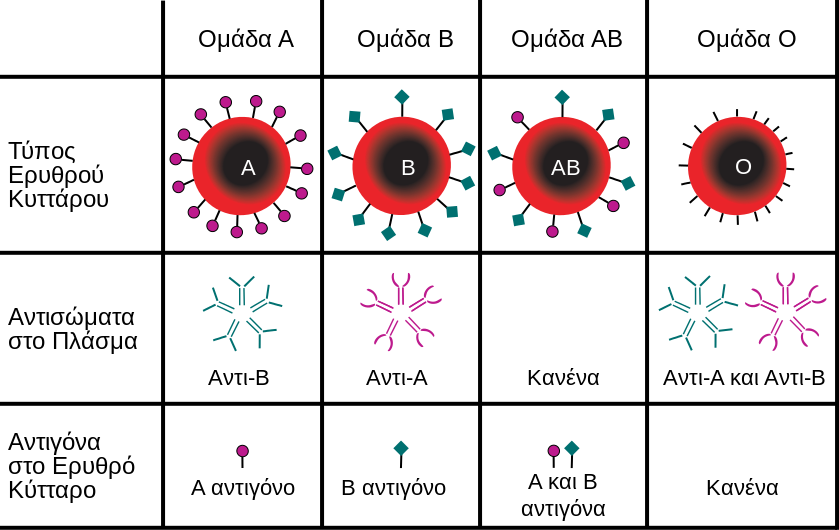
\includegraphics[width=0.7\textwidth]{blood_antibodies_antigons.png}
	    \caption{Αντισώματα και αντιγόνα του αίματος}
	    \label{fig:blood_antibodies_antigons}
	\end{figure}
			
			Στις μεταγγίσεις πρέπει να λαμβάνεται υπόψιν και ένας άλλος παράγοντας, που λέγεται παράγοντας Rhesus, επειδή ανακαλύφθηκε πρώτα στα ερυθρά αιμοσφαίρια του πιθήκου Rhesus Maccacus. Το σύστημα Rhesus είναι το δεύτερο κατά σπουδαιότητα σύστημα ομάδων αίματος μετά το ΑΒΟ. Η γνώση του είναι απαραίτητη για την ασφαλή μετάγγιση αίματος, ενώ είναι το σύστημα, που κυρίως ευθύνεται για την αιμολυτική νόσο του νεογνού. Σήμερα είναι γνωστά περί τα 50 αντιγόνα που ανήκουν στο σύστημα Rhesus. Από αυτά τα πέντε είναι τα πιο κύρια και βασικά. Το κυριότερο αντιγόνο είναι το D και άτομα που το έχουν στα ερυθρά αιμοσφαίρια είναι Rh-Θετικά ή Rh (+), ενώ αυτά που δεν το έχουν είναι Rh-Αρνητικά ή Rh (-). Το αντιγόνο D είναι εξαιρετικά ανοσογόνο (immunogenic) και άτομα Rh-Αρνητικά, όταν εκτεθούν σε αυτό, μπορούν να σχηματίσουν anti-D αντισώματα. Το 85\% των λευκών ανθρώπων έχουν τον παράγοντα αυτόν, δηλαδή είναι Rh-Θετικοί και το 15\% δεν τον έχουν, δηλαδή είναι Rh-Αρνητικοί \cite{Landsteiner01011940}. 

Συμβάντα μπορεί να παρατηρηθούν, αν δεν προσδιοριστεί ο παράγοντας Rhesus, στις εξής περιπτώσεις.
\begin{enumerate}
	\item Σε άτομα στα οποία έγινε μια πρώτη μετάγγιση και στα οποία μια δεύτερη μετάγγιση μπορεί να είναι θανατηφόρα
	\item Στις γυναίκες στις οποίες γίνεται μετάγγιση κατά τη διάρκεια της εγκυμοσύνης τους
	\item Στις γυναίκες που γέννησαν ήδη το πρώτο τους παιδί και στις οποίες μετά από λίγο γίνεται μετάγγιση
	\item Στα έμβρυα λόγω του παράγοντα Ρέζους μπορεί να προκληθεί μια πολύ σοβαρή πάθηση που λέγεται ερυθροβλάστωση των εμβρύων (αν η μητέρα είναι Ρέζους αρνητική, ο πατέρας Ρέζους θετικός και το έμβρυο επίσης Ρέζους θετικό). Κατά την αρρώστια αυτή τα αιμοσφαίρια του εμβρύου συγκολλούνται και προκαλείται τελικά ο θάνατος του. Μπορεί να σωθεί μόνο, αν γεννηθεί ζωντανό και γίνει αλλαγή του αίματος του (αφαιμαξομετάγγιση) με άλλο αίμα Ρέζους αρνητικό
\end{enumerate}

Βάση όσων έχουν αναφερθεί παραπάνω, στο σχήμα \ref{fig:blood_compatibility} βλέπουμε τη συμβατότητα των διαφόρων συνδυασμών.
	\begin{figure}[h!]
	    \centering
	    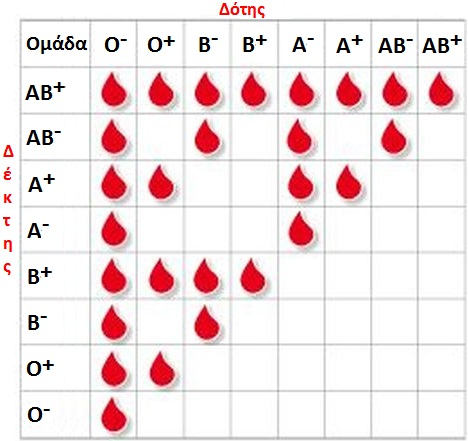
\includegraphics[width=0.5\textwidth]{blood_compatibility.jpg}
	    \caption{Συμβατότητα ομάδων αίματος}
	    \label{fig:blood_compatibility}
	\end{figure}
	
	Από την άλλη μεριά η μετάγγιση πλάσματος έχει τους αντίθετους κανόνες αφού τα αντιγόνα βρίσκονται στο πλάσμα. Για παράδειγμα ένας ασθενής με τύπο αίματος O μπορεί να λάβει πλάσμα από τις ομάδες αίματος A,B και ΑΒ αφού το πλάσμα του τύπου Ο περιέχει αντιγόνα και της Α και της Β. Στον πίνακα \ref{tab:plasma_compatibility} βλέπουμε τη συμβατότητα πλάσματος των διάφορων συνδυασμών.
\begin{table}[H]
	\centering
	\begin{tabular}{l|llll}
		Ασθενής & \multicolumn{4}{l}{Αιμοδότης} \\ \hline
			& Ο     & Α     & Β     & ΑΒ    \\
		Ο       & Ναι   & Ναι   & Ναι   & Ναι   \\
		Α       & Όχι   & Ναι   & Όχι   & Ναι   \\ 
		Β       & Όχι   & Όχι   & Ναι   & Ναι   \\
		ΑΒ      & Όχι   & Όχι   & Όχι   & Ναι  
	\end{tabular}
	\caption{Συμβατότητα πλάσματος}
	\label{tab:plasma_compatibility}
\end{table}
	Σε αυτό το σημείο, θα πρέπει να αναφερθεί ότι η κατανομή του πληθυσμού στις διάφορες ομάδες αίματος δεν είναι ισόποση. Στο σχήμα \ref{fig:blood_distribution} βλέπουμε την κατανομή σε επιλεγμένες χώρες.
\begin{figure}[h!]
	    \centering
	    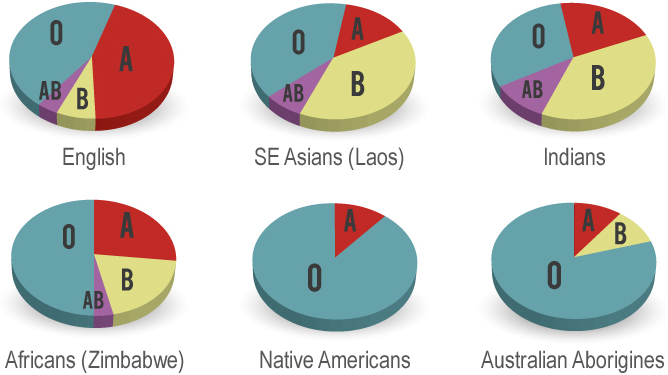
\includegraphics[width=0.7\textwidth]{blood_distribution.jpg}
	    \caption{Κατανομή ομάδων αίματος}
	    \label{fig:blood_distribution}
\end{figure}	

	\subsection{Αιμοδοσία}
	Με τον όρο αιμοδοσία, εννοούμε τη χορήγηση αίματος από υγιείς δότες σε άτομα στα
οποία η κατάσταση της υγείας τους απαιτεί μετάγγιση. Κατ' επέκταση με τον όρο αιμοδοσία εννοούμε την όλη οργάνωση που ασχολείται με τη λήψη, επεξεργασία, συντήρηση και διάθεση του αίματος και των παραγώγων του \cite{bloodDonationDefinition}. Η αιμοδοσία καλείται εθελοντική, επειδή αφορά σε πράξη που εκτελεί κάποιος με τη θέλησή του και με μοναδικά κίνητρα τα αισθήματα αλληλεγγύης και αλτρουισμού \cite{1973}. 

Ως επιστημονικός τομέας, η αιμοδοσία αποτελεί ιδιαίτερο κλάδο της αιματολογίας με τεράστια ανάπτυξη τα τελευταία 20 χρόνια. Η καθιέρωση της αιμοδοσίας ως εξειδικευμένου τομέα, καθώς και η αλματώδης ανάπτυξή της, οδήγησαν στην ανάγκη να πλαισιώνεται από ιατρικό, νοσηλευτικό και τεχνικό προσωπικό υψηλής στάθμης με εξειδίκευση στον τομέα της αιμοδοσίας.  
	
	Η μετάγγιση αίματος γίνεται τακτικά σε εγχειρήσεις, τραυματίες, γαστρορραγίες και σε τοκετούς για την αναπλήρωση της απώλειας σημαντικής ποσότητας αίματος. Στις περισσότερες περιπτώσεις η μετάγγιση αίματος χρησιμοποιείται ως προσωρινή μορφή θεραπείας. Βέβαια, υπάρχουν και περιπτώσεις όπου ο ασθενής χρειάζεται μεταγγίσεις αίματος εφόρου ζωής. Μερικές ευρέως γνωστές ασθένειες που απαιτούν κάτι τέτοιο είναι η Β-Θαλασσαιμία (η Ελλάδα έχει τα υψηλότερα ποσοστά), αιμοφιλία και λευχαιμία \cite{thalassaemiaLongTerm}.

	Αν και υπάρχουν κάποιες περιπτώσεις οι οποίες απαιτούν μετάγγιση ολικού αίματος, η πλειονότητα του αίματος διασπάται μετά τη δωρεά και τα απαιτούμενα προϊόντα αίματος μεταφέρονται στον ασθενή. Ακολουθώντας την παραπάνω προσέγγιση, από τη μία μεριά ο ασθενής δεν λαμβάνει περιττά συστατικά και από την άλλη μεριά από μία μονάδα ολικού αίματος μπορούν να επωφεληθούν περισσότεροι του ενός ατόμου. Η διάρκεια ζωής των διαφόρων συστατικών του αίματος φαίνεται στον πίνακα \ref{tab:blood-shelf-life} παρακάτω \cite{Basu2014}:
	
\begin{table}[H]
		\centering
		\begin{tabular}{l|ll}
			\hline
			Συστατικό          & Διάρκεια  & Θερμοκρασία \\ \hline
			Ολικό αίμα         & 24 ώρες   & 20-24       \\
			Ερυθρά αιμσοφαίρια & 42 μέρες  & 4           \\
			Αιμοπετάλια        & 3-5 μέρες & 20-24       \\
			Πλάσμα             & 1 χρόνος  & -18        
		\end{tabular}
		\caption{Διάρκεια ζωής συστατικών αίματος}
		\label{tab:blood-shelf-life}
\end{table}	

Από τα δεδομένα του παραπάνω πίνακα γίνεται εύκολα εμφανές ότι είναι προτιμότερο να αποθηκεύονται τα συστατικά του αίματος πάρα το ολικό αίμα, ενώ παράλληλα γίνεται εμφανής η ανάγκη για συνεχή παροχή αιμοδοσιών.
	
	 Το αίμα που χρησιμοποιείται στις μεταγγίσεις πρέπει να προέρχεται από υγιή άτομα. Το αίμα δεν είναι μόνο ζωντανός ιστός, αλλά έχει επιπλέον την ιδιότητα να ανανεώνεται και τα υγιή άτομα διαθέτουν μηχανισμούς αύξησης της παραγωγής αίματος. Έτσι με την αιμοδοσία προσφέρεται εύκολα το δώρο της ζωής χωρίς τον φόβο ότι η τακτική αιμοδοσία θα προκαλέσει εξασθένηση του οργανισμού και θα οδηγήσει σε αδυναμία η επιτάχυνση της γήρανσης.
	 
	Στόχος είναι οι εθελοντές, που πληρούν τα κριτήρια για αιμοδοσία να γίνονται τακτικοί αιμοδότες, δηλαδή να πραγματοποιούν δωρεά αίματος αρκετές φορές το χρόνο και να παραμένουν στον κατάλογο των ενεργών αιμοδοτών για πολλά χρόνια. Η διατήρηση ενός υψηλού επιπέδου ποιότητας παρεχομένων υπηρεσιών στην υπηρεσία αιμοδοσίας συνίσταται στην προτεραιότητα ικανοποίησης των αναγκών και των προσδοκιών των εθελοντών αιμοδοτών. Ωστόσο είναι σημαντικό να επισημάνουμε ότι μια επένδυση στην προσέλκυση και στη διατήρηση εθελοντών θα αποδώσει ασφαλή αποθέματα αίματος και προστασία της υγείας τόσο στον δότη όσο και στον λήπτη. Επιπλέον θα υπάρχει και σημαντική εξοικονόμηση κόστους για την υπηρεσία μέσω της μείωσης του αριθμού μονάδων αίματος που πρέπει να απορριφθούν λόγω της ανεύρεσης θετικών δεικτών λοιμωδών νοσημάτων. 
	
	Η προσέλκυση και η διατήρηση των εθελοντών αιμοδοτών είναι μια δυναμική λειτουργία που σχεδιάζεται κάθε φορά ανάλογα με τη μελέτη και την ανάλυση των παραμέτρων της συγκεκριμένης κοινωνικής ομάδας που απευθυνόμαστε σε σχέση με την αξιολόγηση και εκτίμηση των αναγκών σε αίμα και την υπάρχουσα κατάσταση στον χώρο.
		\subsubsection{Διαδικασία της Αιμοδοσίας}
		
		 Η επιλογή των αιμοδοτών γίνεται από άρτια εκπαιδευμένο και επαγγελματικά καταρτισμένο προσωπικό που έχει ως σκοπό την ασφάλεια τόσο του αιμοδότη όσο και του δέκτη. Στην είσοδο της αιμοδοσίας υπάρχουν ειδικά έντυπα αυτοαποκλεισμού, τα οποία καλούνται να διαβάσουν όλοι οι άνθρωποι που προσέρχονται προκειμένου να προσφέρουν αίμα \cite{diadikasiaAimodosias}. Στην συνέχεια αν ο δυνητικός αιμοδότης κρίνει ότι πληροί τα κριτήρια αποδοχής και δεν ισχύει κάποιο από τα κριτήρια αποκλεισμού για την περίπτωση του, θα πρέπει να συμπληρώσει το ερωτηματολόγιο του αιμοδότη \cite{ekeaQuestionnaire} (περισσότερα στο Παράρτημα Α). Το προαναφερθέν ερωτηματολόγιο είναι εμπιστευτικό διασφαλίζοντας το ιατρικό απόρρητο και θα πρέπει να συμπληρώνεται από τον αιμοδότη κάθε φορά που θέλει να δώσει αίμα. Ο αιμοδότης έχει τη δυνατότητα να συζητήσει με τον ιατρό προβλήματα υγείας ή άλλους λόγους που θέτουν ενδεχομένως σε κίνδυνο την ασφάλεια του ίδιου ή του δέκτη.
		 
		 Στην συνέχεια ο αιμοδότης εξετάζεται για αρτηριακή πίεση, σφυγμό, βάρος, αιματοκρίτη ή αιμοσφαιρίνη, πιθανές δερματικές αλλοιώσεις στο σημείο της φλεβοκέντησης, καθώς και σχετικά με τη φυσική του κατάσταση. Ο γιατρός της αιμοδοσίας, εφόσον συλλέξει τις απαραίτητες πληροφορίες και λαμβάνοντας υπόψιν τις απαντήσεις στο ερωτηματολόγιο του αιμοδότη, κρίνει αν κάποιος, ο οποίος προσέρχεται στην υπηρεσία αιμοδοσίας, είναι σε θέση να προσφέρει αίμα. Την τελική ευθύνη για την επιλογή του αιμοδότη την επωμίζεται ο ιατρός της αιμοδοσίας.
		 
		Πρέπει να σημειωθεί, σε αυτό το σημείο, πως είναι απαραίτητη η έγγραφη συγκατάθεση του αιμοδότη ότι δέχεται να αιμοδοτήσει και να εξεταστεί το αίμα του για μεταδοτικά νοσήματα. Σε περίπτωση απόρριψης δίνονται οι απαραίτητες ιατρικές πληροφορίες και εξηγήσεις οι οποίες αφορούν στον λόγο και στη διάρκεια αποκλεισμού (για περισσότερα βλ: \ref{sssec:donor_screening}).
		
		Αφού κριθεί ότι ο αιμοδότης πληροί τις προϋποθέσεις, οδηγείται στην ειδική καρέκλα της αιμοδοσίας, γίνεται περίδεση του βραχίονα και καλή αντισηψία στην περιοχή της φλεβοκέντησης. Κατά τη διαδικασία της αιμοληψίας συστήνεται στον αιμοδότη να ανοιγοκλείνει τη γροθιά του, ώστε να διευκολύνεται η ροή του αίματος. Λαμβάνονται 450ml αίματος. Ο όγκος του αίματος, που προσφέρεται, αναπληρώνεται μέσα σε 24 ώρες μετά την αιμοδοσία.
		
		Μετά την αιμοληψία, το αίμα συλλέγεται σε ειδικούς σάκους, που περιέχουν αντιπηκτικές και άλλες ουσίες, οι οποίες βοηθούν στην άριστη διατήρηση του αίματος. Πριν αφαιρεθεί η βελόνα λαμβάνονται δείγματα για τις εξετάσεις, όπως προβλέπεται από το νόμο. Στο τέλος, ο αιμοδότης καλείται να παραμείνει καθιστός για λίγη ώρα, καθώς παράλληλα σε κάποια κέντρα του προσφέρεται χυμός και κάποιο μικρό πρόχειρο γεύμα.
		
		Πρόκειται για μια ανώδυνη διαδικασία. Μοναδικό ενόχλημα είναι ένας μικρός πόνος από τη βελόνα. Η αιμοδοσία είναι ακίνδυνη για τον αιμοδότη. Η περίπτωση να μολυνθεί ο αιμοδότης από AIDS ή άλλο μεταδιδόμενο νόσημα είναι μηδενική, αφού οι βελόνες που χρησιμοποιούνται είναι μιας χρήσης και αποστειρωμένες.
		
		Η αιμοδοσία διαρκεί περίπου δέκα λεπτά. Για την όλη διαδικασία, από τη συμπλήρωση του ερωτηματολογίου μέχρι να φύγει ο αιμοδότης, απαιτείται περίπου μισή ώρα \cite{diadikasiaAimodosias}.
	\subsection{Εθελοντές αιμοδότες}
		\subsubsection{Κριτήρια επιλογής αιμοδοτών} \label{sssec:donor_screening} 
			Αίμα μπορούν να δώσουν όλοι οι υγιείς άντρες και γυναίκες ηλικίας 18 - 65 ετών οι οποίοι έχουν σωματικό βάρος μεγαλύτερο των 50 κιλών, κάθε 3 - 4 μήνες. Βασικός στόχος και υποχρέωση των υπηρεσιών μετάγγισης αίματος είναι να συλλέξουν αίμα από υγιείς αιμοδότες, ώστε αφενός να προφυλαχθεί η δική τους υγεία και αφετέρου να προστατευθεί ο αιμολήπτης ασθενής από τη μετάδοση ασθενειών ή φαρμακευτικών ουσιών που μπορεί δυνητικά να είναι βλαβερά για την υγεία του. Ο υποψήφιος αιμοδότης κατά τη λήψη του ιστορικού πρέπει να αναφέρει τυχόν συμπτώματα, ώστε να βοηθήσει το ιατρικό προσωπικό να κρίνει με ασφάλεια την πιθανότητα κινδύνου. Κάθε πρόβλημα υγείας που ενδεχομένως έχει ο υποψήφιος αιμοδότης, πρέπει να συζητείται με τον υπεύθυνο γιατρό της αιμοδοσίας, ο οποίος και κρίνει τελικά για τη καταλληλότητα της αιμοληψίας. Η διαδικασία θα πρέπει να είναι τέτοια έτσι ώστε να εξασφαλίζεται ασφαλή αιμοδοσία και παροχή αίματος αλλά και να μην απορρίπτονται υγιείς αιμοδότες οι οποίοι θα μπορούσαν να συνεισφέρουν \cite{bloodDonorSelection}.
			
			Ο αιμοδότης πρέπει να είναι σε καλή υγεία και απαλλαγμένος από μεταδοτικές ασθένειες. Όμως κάθε άνθρωπος είναι επιρρεπής σε μικρο-αδιαθεσίες. Αυτές είναι πόνοι κάθε είδους, ακμή, πονόλαιμοι και δυσπεψία. Όλα αυτά δεν αποτελούν στοιχεία απόρριψης του αιμοδότη. Εάν ο δότης υποβάλλεται σε φαρμακευτική αγωγή ή έχει υποβληθεί στο άμεσο παρελθόν, πρέπει να σημειωθούν τα παρακάτω σχετικά με τα φάρμακα που παίρνει. Η ποσότητα του φαρμάκου, δηλαδή η πυκνότητα του φαρμάκου στον οργανισμό του δότη και η ταχύτητα απορρόφησης ή η αποβολή του. Το φάρμακο μπορεί να έχει δυσμενή επίπτωση στον δέκτη εφόσον η περιεκτικότητα του φαρμάκου στον δότη είναι αυξημένη. Εάν ο δέκτης είναι αλλεργικός σ' αυτό το φάρμακο ή εάν ο δέκτης είναι έγκυος γυναίκα μπορεί να προκληθεί μέχρι και τερατογένεση. Το φάρμακο μπορεί να διαταράξει το αίμα του δότη, π.χ. τη λειτουργικότητα των αιμοπεταλίων. Παρόλο ότι τα φαινόμενα αυτά έχουν αναγνωριστεί, η συχνότητά τους δεν μελετήθηκε ακόμη καλά. Εάν λοιπόν ο αιμοδότης λαμβάνει φάρμακα, δεν σημαίνει ότι αναγκαστικά δεν μπορεί να προσφέρει αίμα. Σε κάθε περίπτωση όμως είναι ορθό να ενημερώνεται ο γιατρός και το προσωπικό για τα φάρμακα που λαμβάνει και ανάλογα θα κριθεί εάν μπορεί να προσφέρει αίμα \cite{bloodDonorSelection}. 
			
		Υπάρχουν καταστάσεις και νοσήματα που αποκλείουν δια παντός την αιμοδοσία, όπως είναι το AIDS, οι ηπατίτιδες, η ελονοσία, η χρήση ενδοφλεβίων ναρκωτικών, οι κακοήθειες, η υπέρταση, ο σακχαρώδης διαβήτης ή σοβαρά χρόνια νοσήματα. Στις περισσότερες περιπτώσεις, όμως, ο αποκλεισμός είναι μόνο πρόσκαιρος.  Ο αποκλεισμός αυτός γίνεται για να μην επιβαρυνθεί η υγεία του αιμοδότη και για να διασφαλιστεί η ποιότητα του αίματος που θα μεταγγιστεί στο λήπτη. Μελέτες έχουν δείξει ότι ο προσωρινός αποκλεισμός από την αιμοδοσία έχει έντονο αρνητικό αντίκτυπο στη μελλοντική επιστροφή του αιμοδότη \cite{Custer2011}\cite{Custer2007}. Για αυτό είναι υψίστης σημασίας να δίνονται ξεκάθαρα διαστήματα αποκλεισμού και να ενθαρρύνονται οι εθελοντές να επιστρέψουν μετά το πέρας αυτού του διαστήματος. Στο σύστημα που προτείνουμε στην παρούσα διπλωματική έχει γίνει μέριμνα για τέτοιες περιπτώσεις και υλοποιήθηκε ένα σύστημα κατάλληλων ειδοποιήσεων.
		
		Εκτός από τις γενικές αυτές αρχές και επειδή οι λεπτομέρειες στις ενδείξεις αναπροσαρμόζονται, ο υποψήφιος αιμοδότης πρέπει να συμβουλεύεται το προσωπικό της αιμοδοσίας που είναι το πλέον αρμόδιο για την επιλογή των αιμοδοτών.
		\subsubsection{Κατηγορίες αιμοδοτών}
			Οι αιμοδότες μπορούν να χωριστούν σε τρεις μεγάλες κατηγορίες:
\begin{enumerate}
	\item Οι εθελοντές αιμοδότες (Volunteer Donors - VDs) οι οποίοι αιμοδοτούν με δική τους πρωτοβουλία καθαρά για ανθρωπιστικούς λόγους, χωρίς να λαμβάνουν κάποιο οικονομικό αντάλλαγμα ή οτιδήποτε που θα μπορούσε να θεωρηθεί ως αντικαταστατό του χρήματος.
	\item Οι δότες αντικατάστασης (Replacement Donors - RDs), οι οποίοι αιμοδοτούν προκειμένου να καλύψουν τις ανάγκες που προκύπτουν από συγγενείς ή φίλους οι οποίοι νοσηλεύονται.
	\item Δότες αίματος επί πληρωμή οι οποίοι λαμβάνουν πληρωμή από την οικογένεια η οποία δεν μπορεί να παρέχει η ιδία δότη αντικατάστασης για το συγγενικό τους πρόσωπο.
\end{enumerate} 

		Σε αυτό το σημείο πρέπει να αναφέρουμε, ότι η τρίτη κατηγορία αιμοδοτών εμφανίζεται μόνο σε τριτοκοσμικές χώρες και κυρίως σε χώρες της Αφρικής. Στατιστικά στοιχεία έχουν δείξει ότι οι τακτικοί εθελοντές αιμοδότες (VDs) σχετίζονται με ασφαλέστερες παροχές αίματος σε σχέση με τους δότες αντικατάστασης όσον αφορά στις μεταδιδόμενες κατά την μετάγγιση ασθένειες \cite{Liu1998}.

		Στοιχεία του Παγκόσμιου Οργανισμού Υγείας (WHO) και του Συμβουλίου της Ευρώπης υποδεικνύουν ότι το αίμα και τα παράγωγα του αίματος θα πρέπει να συλλέγονται αποκλειστικά από τακτικούς μη αμειβόμενους εθελοντές \cite{VOX:VOX5295}. Τα συστήματα αιμοδοσίας τα οποία στηρίζονται στους εθελοντές αιμοδότες οι οποίοι δίνουν αίμα σε σταθερή βάση έχουν τη δυνατότητα να διαχειριστούν καλύτερα τις παροχές αίματος και να προγραμματίσουν τις μεταγγίσεις, επιταχύνοντας την όλη διαδικασία. Τέλος, από ηθική άποψη, δεν είναι σωστό να αναγκάζονται οι συγγενείς ενός ασθενούς σε ανάγκη, να αναζητούν κάτω από ψυχολογική πίεση άτομα για να προσφέρουν αίμα προκειμένου να καλυφθούν οι ανάγκες του δικού τους ανθρώπου.

		Οι εθελοντές αιμοδότες (VDs) μπορούν να χωριστούν περαιτέρω στις ακόλουθες κατηγορίες \cite{karabaggeli-blatsa}:
		\begin{enumerate}
			\item Στους συστηματικούς και αυτόνομους, οι οποίοι προσέρχονται να αιμοδοτήσουν με δική τους αποκλειστικά πρωτοβουλία.
			\item Στους οργανωμένους σε συλλόγους ή τράπεζες αίματος, που καλούνται να δώσουν αίμα.
			\item Στους περιστασιακούς, που απαντούν σε εκκλήσεις ραδιοφωνικών σταθμών και άλλων μέσων.
			\item Στους εποχιακούς, που δίνουν αίμα κατά την ημέρα της αιμοδοσίας του Δήμου, του πολιτιστικού συλλόγου που ανήκουν και άλλων οργανώσεων.
		\end{enumerate}
		
		Ο πραγματικός βέβαια εθελοντής αιμοδότης είναι εκείνος που προσέρχεται να δώσει αίμα με μοναδικό κίνητρο την κοινωνική αλληλεγγύη και τον αλτρουισμό, δεν τον απασχολεί σε ποιον θα δοθεί το αίμα που πρόσφερε και δεν περιμένει κανένα απολύτως αντάλλαγμα.
				
	\subsection{Εθελοντική αιμοδοσία στην Ελλάδα}
		Στην Ελλάδα το "Εθνικό Κέντρο Αιμοδοσίας" (Ε.ΚΕ.Α) το οποίο στεγάζεται στο Υπουργείο Υγείας και Πρόνοιας αποτελεί το κεντρικό όργανο για την οργάνωση των Υπηρεσιών Αιμοδοσίας. Οι Υπηρεσίες Αιμοδοσίας μπορούν να διαχωριστούν στις παρακάτω τρεις κατηγορίες:
		\begin{enumerate}
			\item Κέντρα Αίματος
			\item Σταθμοί Αιμοδοσίας Α' Τάξης
			\item Σταθμοί Αιμοδοσίας Β' Τάξης
		\end{enumerate}
				 
		 Τα κέντρα Αίματος καλύπτουν τις ανάγκες μιας ευρύτερης γεωγραφικής περιοχής ή μεγάλων πληθυσμιακών ομάδων και εδρεύουν σε νοσοκομεία. Κάθε κέντρο αίματος εκτελεί μοριακούς έλεγχους για τους σταθμούς αιμοδοσίας της περιοχής του (για περισσότερα βλ. παράρτημα \ref{ch:blood_centers}) Η Ελλάδα διαθέτει 4 μεγάλα κέντρα αίματος: 
		\begin{enumerate}
			\item Ε.ΚΕ.Α - Εθνικό κέντρο αιμοδοσίας.
			\item Πανεπιστημιακό Νοσοκομείο ΑΧΕΠΑ Θεσσαλονίκης.
			\item Πανεπιστημιακό Νοσοκομείο Ρίο Πατρών.
			\item Πανεπιστημιακό Νοσοκομείο Βενιζέλειο Ηρακλείου Κρήτης.
		\end{enumerate}				 
		 
		 Οι σταθμοί Αιμοδοσίας Α' Τάξης είναι μικρότερες υπηρεσίες και καλύπτουν τις ανάγκες του νοσοκομείου στο οποίο εδρεύουν και άλλες τοπικές ανάγκες. Οι Σταθμοί Αιμοδοσίας Β' Τάξης καλύπτουν αποκλειστικά τις ανάγκες του νοσοκομείου που στεγάζονται.
		
		Το σύστημα αιμοδοσίας στην Ελλάδα είναι αποκεντρωμένο και αποτελείται από 101 υπηρεσίες αιμοδοσίας υπό την αιγίδα και εποπτεία του Υπουργείου Υγείας\cite{filloKivernisews}. Κάθε υπηρεσία αιμοδοσίας αποτελεί ένα ενσωματωμένο μέρος ενός δημόσιου νοσοκομείου και οι αρμοδιότητές της περιλαμβάνουν α) τη στρατολόγηση νέων αιμοδοτών, β) τη συλλογή και τον έλεγχο του αίματος και γ) και τη διακίνηση του αίματος και των παραγώγων του στις νοσοκομειακές κλινικές \cite{Marantidou2007}.
		
		Σύμφωνα με επίσημα δεδομένου του Υπουργείου Υγείας οι ανάγκες για αίμα το έτος 2014 στην Ελλάδα ήταν 750.000 μονάδες. Ένα σημαντικός παράγοντας ο οποίος αυξάνει σημαντικά τις ανάγκες σε αίμα στην χώρα μας και δικαιολογεί το παραπάνω νούμερο, είναι τα υψηλά ποσοστά μεσογειακής αναιμίας για τα οποία χρειάζονται 144.000 μονάδες αίματος ανά χρόνο. 
		
		Σύμφωνα με στοιχεία που έδωσε στη δημοσιότητα το Εθνικό Κέντρο Αιμοδοσίας (Ε.ΚΕ.Α) κατά την διάρκεια του έτους 2013 έγινε εθελοντική αιμοδοσία 584.088 μονάδων αίματος, εκ των οποίων 254.198 (43.52 \%) προήλθε από τους επονομαζόμενους δότες αντικατάστασης (Replacement Donors - RDs),οι οποίοι αιμοδοτούν προκειμένου να καλύψουν τις ανάγκες που προκύπτουν από συγγενείς ή φίλους. Ένα ποσοστό 54.85 \% δηλαδή 320.411 μονάδες προέρχονται από εθελοντές αιμοδότες (Volunteer Donors - VDs), οι οποίοι αιμοδοτούν με δική τους πρωτοβουλία καθαρά για ανθρωπιστικούς λόγους. Οι υπόλοιπες 9.479 μονάδες (0.016\%) προέρχονται από τις ένοπλες δυνάμεις. Η τελευταία αυτή κατηγορία αιμοδοτών έχει δυνατά κίνητρα να αιμοδοτήσει εθελοντικά, καθώς αποζημιώνονται με άδειες και αποχή από τα καθήκοντά τους. Σε αυτό το σημείο κρίνεται σκόπιμο να αναφερθεί ότι τα τελευταία τρία χρόνια έχει παρατηρηθεί αύξηση στις εθελοντικές αιμοδοσίες. Συγκεκριμένα το 2013 παρασχεθήκανε από εθελοντές αιμοδότες (VDs) 21.234 περισσότερες μονάδες αίματος σε σύγκριση με το 2012 \cite{EKEA}. Παρότι τα παραπάνω νούμερα είναι ενθαρρυντικά και παρότι διακρίνεται μια αυξητική τάση των εθελοντικών αιμοδοσιών, αξίζει να σημειωθεί ότι 24.000 μονάδες αίματος εισήχθησαν από την Ελβετία, προκειμένου να καλυφθούν οι εθνικές ανάγκες για αίμα \cite{Marantidou2007}.
		
		Βάση επισήμων στοιχείων, η Ελλάδα διαθέτει έναν ευρύ κατάλογο αιμοδοτών βάσει του οποίου 6 αιμοδότες αντιστοιχούν σε 100 πολίτες, γεγονός που την κατατάσσει τρίτη ανάμεσα στις χώρες- μέλη της Ευρωπαϊκής Ένωσης όσον αφορά στον αριθμό των ατόμων οι οποίοι έχουν δωρίσει αίμα έστω και μία φορά στη ζωή τους  (Eurobarometer, 2009).  Επίσης, η Ελλάδα έρχεται πρώτη όσον αφορά στους μη αιμοδότες, οι οποίοι όμως έχουν σκεφτεί να δώσουν αίμα (Eurobarometer, 2005). Παρόλα τα στοιχεία αυτά όμως, η Ελλάδα που είναι μία χώρα 11.000.000 κατοίκων, πολύ συχνά βρίσκεται στη δυσάρεστη αλλά αναπόφευκτη θέση να εισάγει αίμα από το εξωτερικό, καθώς ο ετήσιος αριθμός μονάδων αίματος δεν επαρκεί για να καλυφθούν οι ανάγκες της χώρας. Αυτό συμβαίνει λόγω των υψηλών ποσοστών μεσογειακής αναιμίας, οι οποίες αναφέρθηκαν και παραπάνω, αλλά και λόγω του ότι οι ανάγκες αίματος κατά τη διάρκεια διάφορων χειρουργικών επεμβάσεων είναι μεγαλύτερη στην Ελλάδα από ότι σε άλλες χώρες της Κεντρικής και Βόρειας Ευρώπης, όπως προκύπτει από την έρευνα του ασφαλούς και καλού αίματος \cite{Grindon1996} και οι προσπάθειες να ελαχιστοποιηθεί αυτή η αλόγιστη χρήση έχουν αποβεί προς το παρόν άκαρπες. 

Όπως γίνεται εμφανές από τα δεδομένα που παρουσιάσαμε παραπάνω, η Ελλάδα όπως και οι περισσότερες χώρες της Ευρώπης πρέπει να καθορίσουν μια στρατηγική με στόχο την αύξηση των τακτικών εθελοντών αιμοδοτών και κατ' επέκτασιν των μονάδων αίματος που συλλέγονται κάθε χρόνο. Η στρατηγική αυτή θα πρέπει να έχει ως κύριο άξονα την αύξηση των εθελοντών αιμοδοτών (VDs) και σταδιακή απογαλάκτιση από τους δότες αντικατάστασης (RDs) για τους λόγους που αναφέραμε στην παραπάνω ενότητα (κατηγορίες εθελοντών αιμοδοτών).

Η ευρύτατη εφαρμογή των μεταγγίσεων, σε συνάρτηση με τις δυσκολίες εξασφάλισης των απαιτούμενων ποσοτήτων αίματος για την κάλυψη των αναγκών, δημιουργούν ένα οξύ ιατρό-κοινωνικό πρόβλημα το οποίο απασχολεί τους υπεύθυνους φορείς υγείας ανά τον κόσμο. Η έλλειψη αίματος συνεπάγεται αναβολές χειρουργικών επεμβάσεων, παράταση της παραμονής των ασθενών στα νοσοκομεία, απώλεια εισοδημάτων από την επιβράδυνση της θεραπείας, καθώς και ευρύτερες ψυχολογικές και κοινωνικές επιπτώσεις, οι οποίες επιβαρύνουν τόσο τους ίδιους τους ασθενείς, όσο και το οικογενειακό τους περιβάλλον. Η αντιμετώπιση του προβλήματος απαιτεί την εφαρμογή Εθνικής Αιμοδοτικής Πολιτικής, η οποία στηριζόμενη σε αρχές μη κερδοσκοπικού μάρκετινγκ, θα αποσκοπεί κυρίως στην ενημέρωση και στην ευαισθητοποίηση του κοινού ως προς την εθελοντική αιμοδοσία \cite{Politis}\cite{Marantidou2007}.

Επομένως, η προσπάθεια του συστήματος αιμοδοσίας στην Ελλάδα πρέπει να έχει δύο βασικούς στόχους, οι οποίοι και ταυτίζονται με τους στόχους του συστήματος μας όπως περιγράφηκαν στο κεφάλαιο 1 της παρούσας διπλωματική εργασίας.
\begin{enumerate}
	\item Τη συνολική αύξηση των μονάδων αίματος που συλλέγονται για να διασφαλιστεί η αυτάρκεια στην παροχή αίματος 
	\item Τη μετατροπή των αιμοδοτών αντικατάστασης σε τακτικούς εθελοντές αιμοδότες, προκειμένου να αυξηθεί η ασφάλεια του αίματος και να διευκολυνθεί η διαχείριση των διαθέσιμων μονάδων αίματος και των παραγώγων του
	\item Τη στρατολόγηση νέων εθελοντών αιμοδοτών με έμφαση σε άτομα τις νεαρής ηλικίας.
\end{enumerate}

Τέλος, θα πρέπει να τονιστεί η επιτακτική ανάγκη για την πραγματοποίηση τόσο οργανωτικών, όσο και επιστημονικών αλλαγών στη χώρα μας στο εγγύς μέλλον, οι οποίες θα μπορέσουν να οδηγήσουν με γοργούς ρυθμούς, στην επίτευξη του πρωταρχικού στόχου, δηλαδή στην επίτευξη αυτάρκειας σε αίμα και παράγωγα αίματος. Μία επάρκεια, η οποία θα πρέπει να προέρχεται αποκλειστικά και μόνο από Εθελοντική Αιμοδοσία. Στην κατεύθυνση αυτή είναι και το ολοκληρωμένο πληροφοριακό σύστημα που μελετήθηκε και υλοποιήθηκε στην παρούσα διπλωματική εργασία.

%\section{Πληροφοριακά συστήματα αιμοδοσίας}
%	\subsection{Κατασταση στο εξωτερικο}
%		Ανελυσε Καναδα και Ηνωμενο Βασιλειο που εχουν κανει καλη δουλεια
%	\subsection{Αποθήκευση προσωπικών δεδομένων - security}
%		(Ελλάδα και εξωτερικό)
%	\subsection{Επεξεργασια Προσωπικών Δεδομένων}
%	\subsection{Ασφάλεια ιατρικών δεδομένων και προστασία του απορρήτου του
%ασθενούς}
%		τι παιζει με την αρχη προστασιας δεδομενων ; (το αναφεραν στο εθνικο μητρωο αιμοδοτων - μαθε λεπτομερειες!)

\section{Κινδυνοι που προκύπτουν μέσα από αιμοδοσία (ασθένειες, ποσοστά)}


	Ο Παγκόσμιος Οργανισμός Υγείας (WHO) συνιστά την ακόλουθη ολοκληρωμένη στρατηγική με στόχο την προώθηση της ασφάλειας και της άμεσης πρόσβασης σε αίμα με ταυτόχρονη μείωση των κινδύνων που εγκυμονούν στις αιμοδοσίες:
	\begin{enumerate}
	\item Δημιουργία μίας εθνικής, άρτιας οργανωμένης υπηρεσίας αιμοδοσίας, η οποία θα μπορεί να εξασφαλίσει με αξιοπιστία και ασφάλεια τα απαραίτητα αποθέματα αίματος για τις ανάγκες του πληθυσμού.
	\item Συλλογή αίματος μόνο από μη-αμειβόμενους εθελοντές αιμοδότες, οι οποίοι τηρούν όλες τις απαραίτητες προϋποθέσεις και φέρουν χαμηλό κίνδυνο απόκτησης επίφοβων λοιμώξεων.
	\item Πλήρεις και ποιοτικές εξετάσεις όλων των αιμοδοσιών για μεταδοτικές μολύνσεις (όπως HIV, ηπατίτιδα Β, ηπατίτιδα C, σύφιλη και άλλες λοιμώξεις)  καθώς και εξετάσεις για τις ομάδες αίματος και τη συμβατότητα τους.
	\item Μείωση των άσκοπων μεταγγίσεων με κατάλληλη κλινική χρήση του αίματος και με διασφάλιση της ασφαλής χορήγησης τόσο του αίματος και όσο και των παραγώγων του \cite{Bolton-Maggs2013}.
\end{enumerate}

	Οι υπηρεσίες Αιμοδοσίας έχουν καθήκον αφενός μεν την φροντίδα για την ασφάλεια του αιμοδότη, αφετέρου δε την εγγύηση του αίματος και των προϊόντων του αίματος που προορίζονται για μετάγγιση. Για τον σκοπό αυτό έχει δημιουργηθεί και αναπτυχθεί η διαδικασία της αιμοεπαγρυπνησης (heamovigilance).

	\subsection{Haemovigilance}
	
	Με τον όρο αιμοεπαγρύπνηση ορίζουμε ως ένα σύνολο οργανωμένων διαδικασιών επιτήρησης, που σχετίζονται με τα ανεπιθύμητα και μη αναμενόμενα συμβάντα και αντιδράσεις στους δότες και τους λήπτες των προϊόντων του αίματος και με την επιδημιολογική παρακολούθηση των αιμοδοτών \cite{VOX:VOX1442}. Η αιμοεπαγρύπνηση εστιάζει στις επιπλοκές των δωρητών αίματος και στις ανεπιθύμητες αντιδράσεις των ληπτών και συμπεριλαμβάνει όλες τις επιπλοκές της ``γραμμής παραγωγής αίματος, την αναλυτική και αναδρομική καταγραφή των συμβαμάτων και την προοπτική έγκαιρης προειδοποίησης με χρήση ενός συστήματος ταχείας έγερσης συναγερμών. Η αιμοεπαγρύπνηση είναι ένα ισχυρό εργαλείο το οποίο στοχεύει στην βελτίωση της ποιότητας των διαδικασιών μετάγγισης αίματος, δίνοντας προτεραιότητα στην ασφάλεια. Απώτερος στόχος της αιμοεπαγρύπνησης είναι η πρόληψη ανεπιθύμητων συμβαμάτων και αντιδράσεων. Εισαγάγει μεθόδους εντοπισμού σφαλμάτων και αντιδράσεων και συμπεριλαμβάνει συστήματα συναγερμού, συστήματα ιχνηλασιμότητας, συστήματα ειδοποιήσεων και τακτικούς ελέγχους των πρακτικών.
	Οι ουσιαστικοί στόχοι της διαδικασίας της αιμοεπαγρύπνησης είναι οι εξής:
		\begin{itemize}
		\item Να προληφθεί η επανεμφάνιση ανεπιθύμητων συμβαμάτων και αντιδράσεων 
		\item Η βελτίωση της πρακτικής μετάγγισης στα νοσοκομεία με τη λήψη προληπτικών ή διορθωτικών μέτρων όπου επιβάλλεται 
		\item Η ανάπτυξη εθνικών κατευθυντήριων οδηγιών και νοσοκομειακών πρωτοκόλλων 
		\item Η διαμόρφωση αποφάσεων σε εθνικό επίπεδο που αφορούν στην ασφάλεια των μεταγγίσεων 
		\item Η εκπαίδευση των γιατρών που χρησιμοποιούν το αίμα, καθώς και των ασθενών που μεταγγίζονται 
		\end{itemize}

	Απαραίτητη προϋπόθεση για την αποτελεσματική λειτουργία της αιμοεπαγρύπνησης είναι η ύπαρξη συστήματος ιχνηλασιμότητας. Ιχνηλασιμότητα ή ανιχνευσιμότητα (traceability) ορίζεται η ικανότητα πλήρους εντοπισμού καθεμίας μονάδας αίματος ή παραγώγων της από τον δότη μέχρι τον τελικό αποδέκτη. Επιτυγχάνεται  με ακριβείς και πλήρεις διαδικασίες αναγνώρισης κάθε δότη, κάθε συλλεγόμενης μονάδας αίματος, καθώς και όλων των παραγώγων του, τήρησης αρχείων και μέσω πλήρους επαλήθευσης της παροχής και μετάγγισης αίματος.Με καταγραφή και μελέτη των απαραιτήτων  δεδομένων για την ιχνηλασιμότητα παράγουμε στατιστικά στοιχεία τα οποία αφορούν στο  σύνολο των ασθενών που έχουν μεταγγισθεί , στις μονάδες ή στα παραγώγα αίματος που έχουν χρησιμοποιηθεί, στους εθελοντές αιμοδότες που έχουν δώσει τις μονάδες αίματος και στα προϊόντα αίματος που μεταγγίσθηκαν. 
		Τα ανεπιθύμητα συμβάματα τα οποία μπορούν να προκύψουν χωρίζονται στις εξής βασικές κατηγορίες:
		\begin{itemize}
		\item	 Σοβαρή ανεπιθύμητη αντίδραση (Serious Adverse Reaction, SAR)
		 "μια άνευ προθέσεως αντίδραση του δότη ή του ασθενούς που σχετίζεται με τη συλλογή ή τη μετάγγιση αίματος ή παραγώγων του και η οποία είναι θανατηφόρα, απειλητική για τη ζωή, προκαλεί αναπηρία ή ανικανότητα ή έχει ως αποτέλεσμα ή παρατείνει τη νοσηλεία ή τη νοσηρότητα", (Οδηγία 2002/98/ΕΚ)
 		\item Σοβαρό ανεπιθύμητο συμβάν (Serious Adverse Event , SAE)
 		"κάθε ατυχές περιστατικό που σχετίζεται με τη συλλογή, τον έλεγχο, την επεξεργασία, την αποθήκευση και τη διανομή αίματος ή παραγώγου του, που θα μπορούσε να προκαλέσει το θάνατο, να απειλήσει τη ζωή, ή να προκαλέσει αναπηρία ή ανικανότητα ή να έχει ως αποτέλεσμα ή να παρατείνει τη νοσηλεία ή τη νοσηρότητα" , (Οδηγία 2002/98/ΕΚ)
 		\item Παρ’ ολίγον συμβάματα (“near miss” events)
 		 "σφάλματα που αν δεν ανιχνευθούν θα μπορούσαν να οδηγήσουν σε λανθασμένο προσδιορισμό ομάδας αίματος, αποτυχία ανίχνευσης ενός ερυθροκυτταρικού αντισώματος, ή σε διανομή, συλλογή ή χορήγηση εσφαλμένου ή ακατάλληλου προϊόντος αίματος ", (Οδηγός, Συμβούλιο της Ευρώπης, Έκδοση 14) 
 		 \item Σφάλματα των μεταγγίσεων χωρίς συμβάματα (uneventful tranfusion errors)
 		 "η μετάγγιση οποιουδήποτε εσφαλμένου, ακατάλληλου ή μη ενδεικνυόμενου προϊόντος αίματος που δεν προκαλεί βλάβη στον λήπτη" (Οδηγός, Συμβούλιο της Ευρώπης, Έκδοση 14η)
 		 \end{itemize} 
 		 
 	Κάθε σοβαρό ανεπιθύμητο συμβάν θα πρέπει να περιγράφεται αναλόγως. Για τον σκοπό αυτόν, έχει καθιερωθεί μία διεθνώς αποδεκτή κλίμακα ταξινόμησης. Η εύρεση της αιτιακής συσχέτισης μεταξύ ανεπιθύμητης αντίδρασης και μετάγγισης, έχει πολύ μεγάλη σημασία, καθώς έτσι μπορούμε να αναγνωρίσουμε αν ευθύνεται κάποιο συστατικό του αίματος ή όχι. Υπάρχουν πολλοί διαφορετικοί τύποι αντιδράσεων μετάγγισης. Η πιο κοινή υποδιαίρεση που χρησιμοποιείται είναι η ταξινόμηση με βάση την εμφάνιση των αντιδράσεων σε οξείες (λιγότερο από 24 ώρες μετά) και καθυστερημένες (περισσότερο από 24 ώρες μετά την μετάγγιση) αντιδράσεις. Πέραν από τους παραλήπτες αίματος, ανεπιθύμητες καταστάσεις μπορούν να προκύψουν και στους εθελοντές αιμοδότες. Τα αίτια και οι παράγοντες, που προκαλούν επιπλοκές στους αιμοδότες, διαφέρουν από τα αντίστοιχα των αιμοληπτών, και χωρίζονται σε τοπικές αντιδράσεις (κυρίως λόγω της εισαγωγής βελόνας), σε γενικότερες αντιδράσεις και σε διάφορους άλλους τύπους επιπλοκών. Οι επιπλοκές ταξινομούνται σε μία διαφορετική διεθνή κλίμακα, έτσι ώστε να να μπορούν να γίνουν συγκρίσεις και τίθενται τα σημεία στα οποία πρέπει να γίνουν παρεμβάσεις. 
 	
		Όλες οι υπηρεσίες αιμοδοσίας και τα νοσοκομεία, υποχρεώνονται να κοινοποιούν στις αρμόδιες αρχές με κατάλληλη διαδικασία αναφοράς τις σοβαρές ανεπιθύμητες αντιδράσεις και τα συμβάματα τα οποία σχετίζονται με τη μετάγγιση αίματος. Οι αναφορές αυτές περιλαμβάνουν πληροφορίες για την κλινική έκβαση των αντιδράσεων και τα μέτρα που έλαβαν οι υπεύθυνοι, σε σχέση με τα άλλα παράγωγα του αίματος που μεταγγίστηκαν, καθώς και τον προσδιορισμό των σοβαρών συμβάντων εξαιτίας ελαττωματικού προϊόντος, εξοπλισμού, ανθρώπινου λάθους και άλλων προβλημάτων \cite{cite-revekka}. Οι μη σοβαρές αντιδράσεις καθώς και άλλα λάθη τα οποία συμβαίνουν κατά την μετάγγιση αίματος δεν αποτελούν αντικείμενο για αναφορά σύμφωνα με τις οδηγίες της Ευρωπαϊκής Ένωσης.
		
		Για την πλήρη και ορθή γνωστοποίηση όλων των άνωθεν πληροφοριών είναι απαραίτητη η ανάπτυξη ολοκληρωμένων πληροφοριακών συστημάτων αιμοεπαγρύπνησης. Για την εφαρμογή ενός συστήματος αιμοεπαγρύπνησης πρέπει να δημιουργούνται λειτουργικοί σύνδεσμοι μεταξύ των Κλινικών τμημάτων, των Κέντρων Αιμοδοσίας, των νοσοκομειακών υπηρεσιών Αιμοδοσίας και των αρμόδιων εθνικών αρχών. Τα αποτελέσματα της ανάλυσης των δεδομένων που προκύπτουν από τα συστήματα αιμοεπαγρύπνησης πρέπει να ανατροφοδοτούνται περιοδικά σε εκείνους, που παρείχαν τα πρωτογενή δεδομένα και στις αρμόδιες αρχές.
		
	
	\subsection{Υπόσυστηματα Haemovigilance Ελλάδα}
	
	Στην Ελλάδα το αρμόδιο όργανο για την αιμοεπαγρύπνηση είναι το Συντονιστικό Κέντρο Αιμοεπαγρύπνησης (ΣΚΑΕ), το οποίο έχει ιδρυθεί από το Ελληνικό  Κέντρο Ελέγχου και Πρόληψης Νοσημάτων (ΚΕ.ΕΛ.Π.ΝΟ),το 1995. Το ΣΚΑΕ απαρτίζεται από εξειδικευμένο προσωπικό στα θέματα ιατρικής, δημόσιας υγείας, εργαστηριακών ελέγχων, στατιστικών αναλύσεων, εκπαίδευσης και οργάνωσης. Η ευρωπαϊκή προσπάθεια για την προώθηση αυστηρών προτύπων για την ποιότητα στην αιμοδοσία και στις μεταγγίσεις αίματος, και ιδίως για τον περιορισμό των κινδύνων που προκύπτουν σε αυτόν τον τομέα της δημόσιας υγείας, οδήγησαν στην ίδρυση του ΣΚΑΕ, το οποίο αποτελεί ιδρυτικό μέλος του Διεθνούς Δικτύου Αιμοεπαγρύπνησης. 
	Η συλλογή των προς ανάλυση δεδομένων γίνεται με τη δημιουργία δικτύων σε τρία επίπεδα: τοπικό δίκτυο (επίπεδο νοσοκομείων, κέντρων αιμοδοσίας), περιφερειακό δίκτυο (το οποίο έχει έξι βάσεις:  στη Νότια Ελλάδα, στην Ανατολική Ελλάδα, Βόρεια Ελλάδα, Δυτική Ελλάδα, Θεσσαλία και την Κρήτη ) και στο εθνικό δίκτυο (ΣΚΑΕ). Το τελευταίο, κοινοποιεί τα αποτελέσματα στο ΚΕ.ΕΛ.Π.ΝΟ και στο Εθνικό Κέντρο Αιμοδοσίας( Ε.Κ.Ε.Α). Στο σχήμα \ref{fig:SKAE_diagram} βλέπουμε το διάγραμμα οργάνωσης του συνολικού δικτύου.
	
\begin{figure}[h!]
	    \centering
	    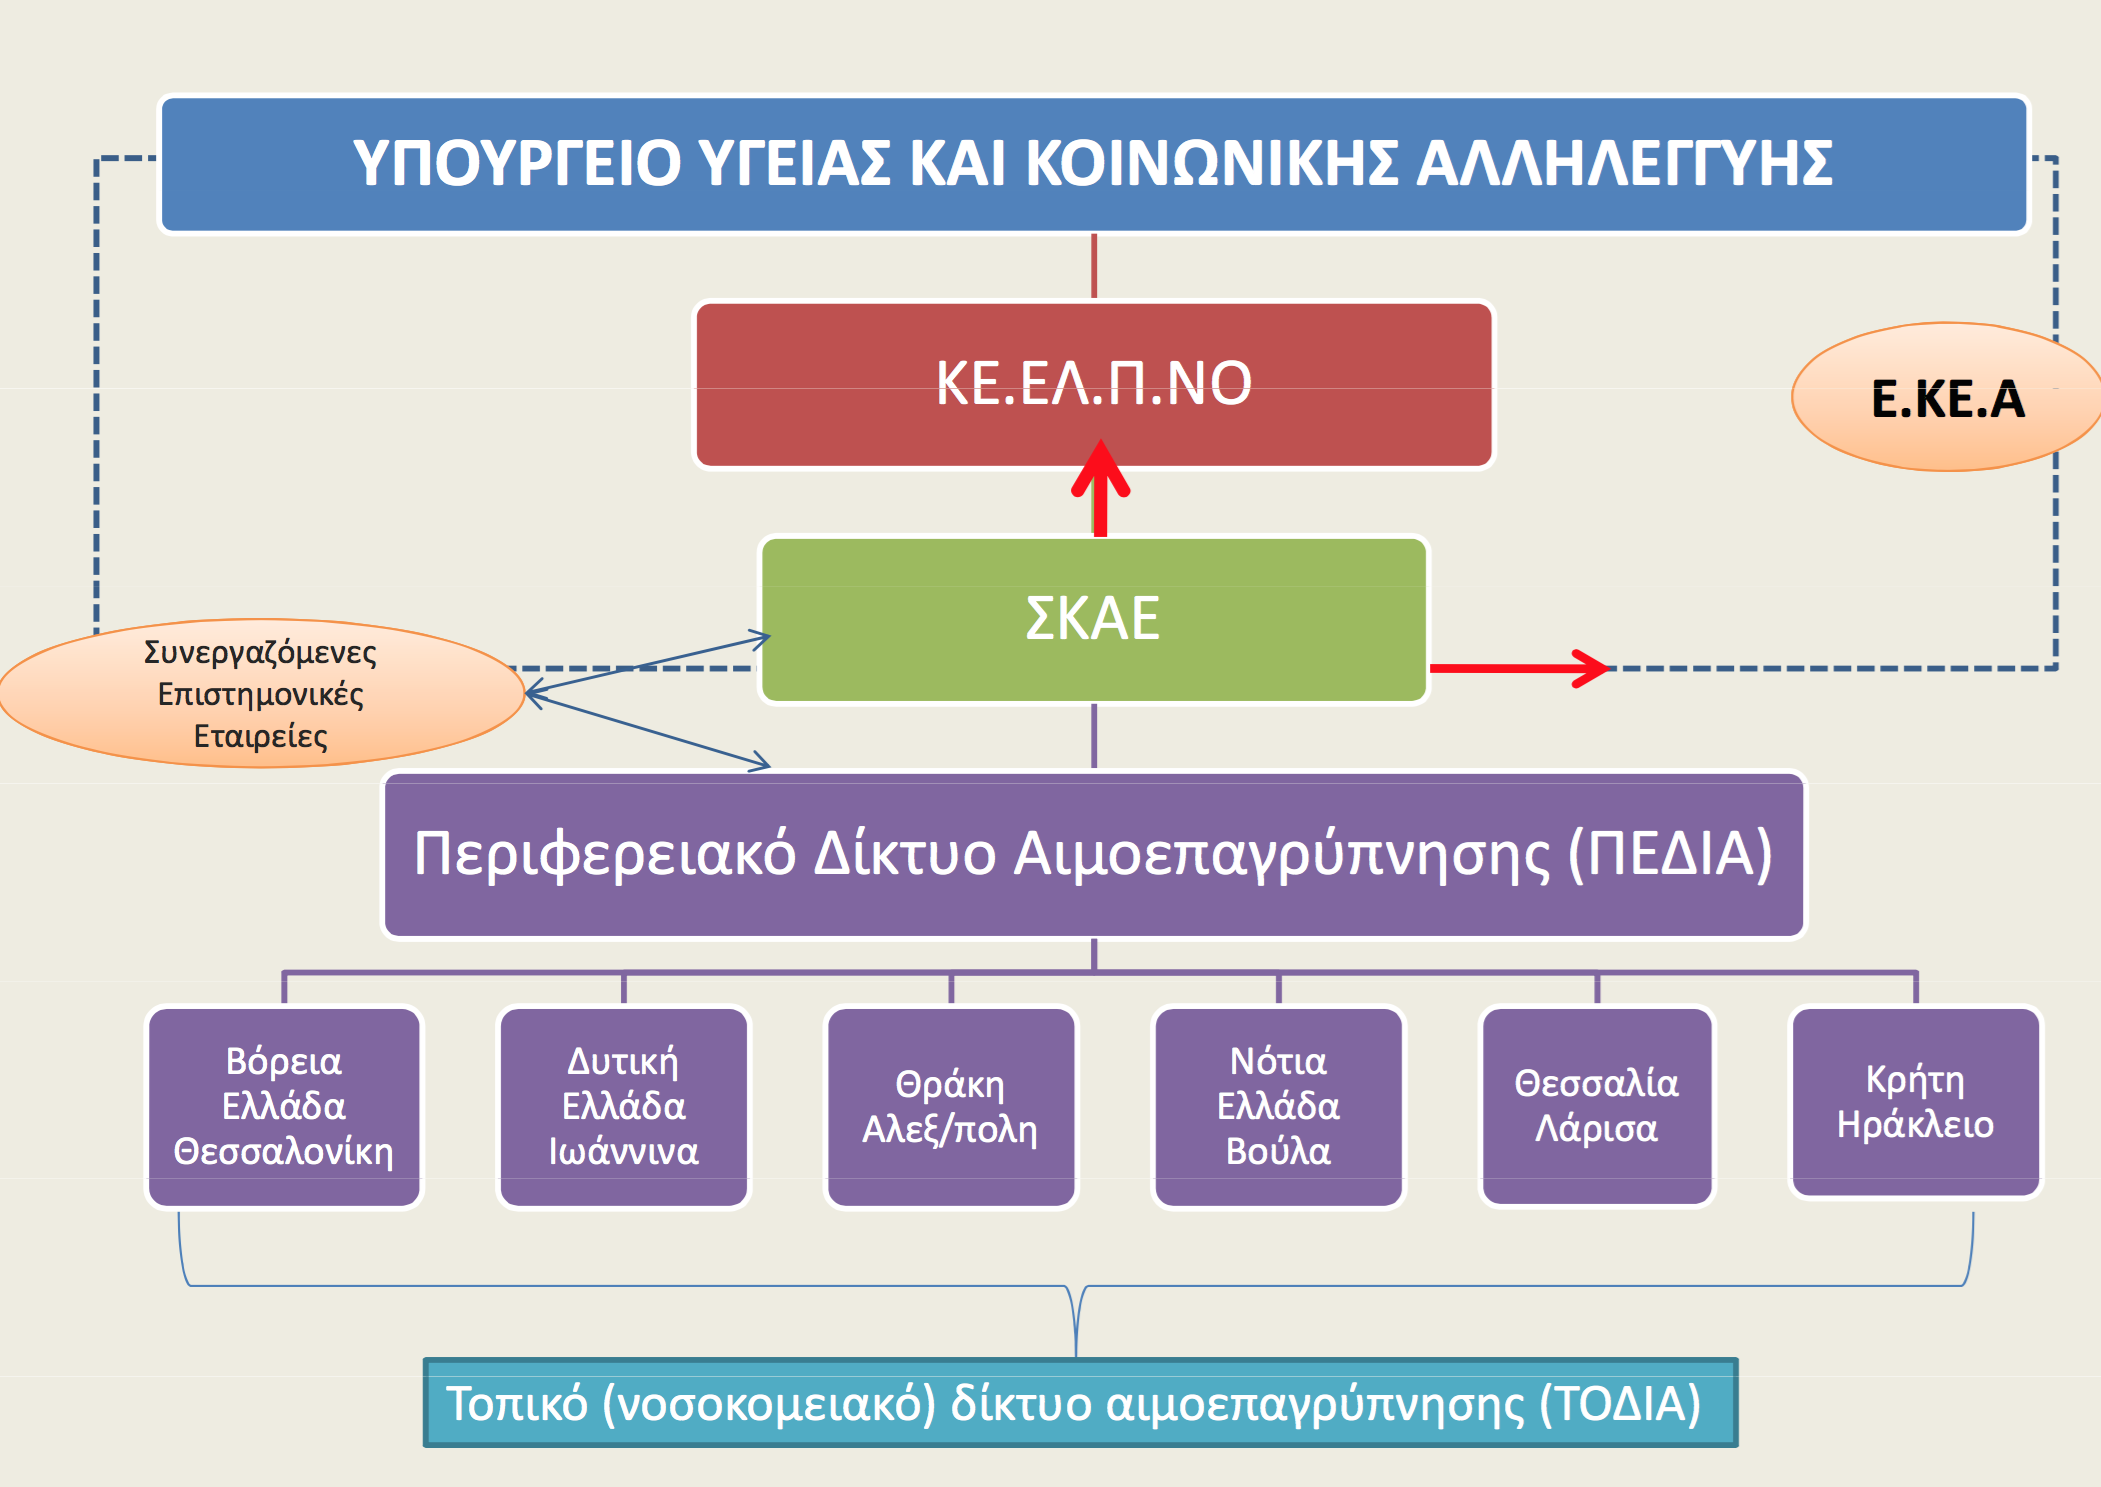
\includegraphics[width=0.7\textwidth]{SKAE_diagram.jpg}
	    \caption{Διάγραμμα λειτουργίας}
	    \label{fig:SKAE_diagram}
\end{figure}	

Οι βασικές λειτουργίες του ΣΚΑΕ είναι οι εξής:
\begin{itemize}
		\item Η συνεχής επιδημιολογική επιτήρηση των λοιμώξεων που μεταδίδονται με το αίμα. Αυτό επιτυγχάνεται με χρήση συστημάτων ανιχνευσιμότητας σε όλα τα στάδια της αιματικής αλυσίδας. Σε περίπτωση εντοπισμού πιθανών μολυσματικών μονάδων, ακολουθεί η άμεση απόσυρση τους. Πραγματοποιούνται διαρκώς αναδρομικοί έλεγχοι, με σκοπό να μειωθούν στο ελάχιστο τα πιθανά λάθη. 
		\item	Η επιδημιολογική επιτήρηση ανεπιθύμητων αντιδράσεων και συμβάντων σχετικών με τη μετάγγιση αίματος. Οι παρατηρήσεις αυτές ακολουθούνται από αναφορές στις αρμόδιες αρχές και διαμόρφωση προτάσεων με αποτελεσματικά διορθωτικά μέτρα, τις οποίες ακολουθούν τα νοσοκομεία και τα κέντρα αιμοδοσίας.  
		\item Η επαγρύπνηση για ανεπιθύμητες αντιδράσεις, ατυχήματα, βλάβες και επιπλοκές στην διάρκεια και μετά από την αιμοδοσία. Άμεση προϋπόθεση του συστήματος επαγρύπνησης είναι η ύπαρξη συστημάτων άμεσης ετοιμότητας εγέρσεων συναγερμών και η αποτελεσματική και αξιόπιστη δυνατότητα διαχείρισης κρίσεων.  Το ΣΚΑΕ ενημερώνει τακτικά την ιατρική κοινότητα για τις εξελίξεις με δημοσιεύσεις και εκδόσεις. 
		\end{itemize}
Το ΣΚΑΕ έχει αναπτύξει πλήρεις και αποτελεσματικές μεθόδους εργασίας, με βάση τις κατευθυντήριες οδηγίες της Ευρωπαϊκής Ένωσης και του Διεθνούς Οργανισμού υγείας(WHO). 

	Όσον αφορά στις λοιμώξεις που μεταδίδονται με το αίμα εφαρμόζεται αναλυτική καταγραφή των οροθετικών αιμοδοτών για HIV, HBV, HCV, σύφιλη, HTLV καθώς και ανάλυση των επιδημιολογικών δεδομένων σε σχέση με τις μονάδες αίματος, την Υπηρεσία Αιμοδοσίας, τα δημογραφικά χαρακτηριστικά των αιμοδοτών (φύλο, ηλικία, τόπος διαμονής, οικονομικό και μορφωτικό επίπεδο), την κατηγορία αιμοδοτών (εθελοντές, συγγενείς, στρατιώτες) και την αιμοδοτική συχνότητα (αιμοδότες πρώτης φοράς, σποραδικοί και τακτικοί). Επιπλέον καταγράφονται αναλυτικά τα δεδομένα για ποιοτικούς ελέγχους, πιστοποιήσεις ποιότητας, δείκτες συλλογής και ελέγχου του αίματος ανά Υπηρεσία Αιμοδοσίας και διαχείρισης ανθρώπινου δυναμικού. Με βάση τους εγγεγραμμένους αιμοδότες πραγματοποιείται συνεχής παρακολούθηση και χαρτογράφηση των ρετροϊκών λοιμώξεων και των ηπατιτίδων στον αιμοδοτικό πληθυσμό. Οι μέθοδοι ορολογικού και μοριακού ελέγχου του αίματος για λοιμώξεις διευρύνονται διαρκώς. Πραγματοποιείται πλήρης καταγραφή δεδομένων για ποιοτικό έλεγχο, πιστοποίηση ποιότητας, δείκτες συλλογής και ελέγχου του αίματος ανά Υπηρεσία Αιμοδοσίας και διαχείρισης ανθρώπινου δυναμικού. Το ΣΚΑΕ έχει καθιερώσει πρωτόκολλα ανιχνευσιμότητας για λοιμώξεις που αναφέρονται ύστερα από μετάγγιση αίματος καθώς και πρωτόκολλα για αναδρομικό έλεγχο των ληπτών δυνητικά μολυσμένου αίματος, τα οποία είναι καθολικά και χρησιμοποιούνται σε όλες τις υπηρεσίες υγείας. Τέλος διεξάγονται διαρκώς μελέτες κόστους – ωφέλειας για τα μέτρα πρόληψης της διασποράς λοιμωδών νόσων με το αίμα και τα προϊόντα του αίματος καθώς και έρευνα πάνω στις νέες λοιμώξεις (Ηπατίτιδα Ε κλπ). 

	Στον τομέα των ανεπιθύμητων αντιδράσεων και των ανεπιθύμητων συμβάντων κατά και μετά την αιμοδοσία καταγράφονται αναλυτικά όλες οι ανεπιθύμητες αντιδράσεις και τα συμβάντα που προκύπτουν κατά την αιμοδοσία εθελοντών και με βάση αυτά τα καταγεγραμμένα γεγονότα αναλύονται οι πληροφορίες που προκύπτουν σχετικά με τον τύπο και τη σοβαρότητα των αντιδράσεων/ συμβαμάτων. Με βάση τις αναλύσεις αυτές προκύπτουν κάποια συμπεράσματα και προτάσεις για βελτίωση της ποιότητας των αιμοδοσιών και δίνονται κατευθυντήριες αρχές στα νοσοκομεία και στα αιμοδοτικά κέντρα.
	
	Οι μέθοδοι εργασίας αναφορικά με τις ανεπιθύμητες αντιδράσεις και τα ανεπιθύμητα συμβάντα σχετικά με τη μετάγγιση αίματος και προϊόντων αίματος περιλαμβάνουν σε πρώτο στάδιο την καταγραφή ανεπιθυμήτων αντιδράσεων, που σχετίζονται με λοιμογόνους παράγοντες (ιογενείς, βακτηριακοί, παρασιτικοί παράγοντες) καθώς και αυτών που σχετίζονται με μη λοιμογόνους παράγοντες, ανεξάρτητα από την σοβαρότητα των αντιδράσεων. Επιπλέον καταγράφονται τα ανεπιθύμητα σοβαρά και «παρ’ ολίγον» συμβάματα και τα σφάλματα των μεταγγίσεων χωρίς σύμβαμα», που μπορεί να επηρεάσουν την ασφάλεια και την ποιότητα του μεταγγιζόμενου προϊόντος αίματος, σε όλες τις διαδικασίες της συλλογής, του ελέγχου, της επεξεργασίας, της αποθήκευσης και της διανομής προϊόντων αίματος. Το ΣΚΑΕ διαμορφώνει τα δελτία αναφοράς των ανεπιθύμητων αντιδράσεων και ανεπιθύμητων συμβάντων και τις οδηγίες διερεύνησης και αντιμετώπισης τους , σύμφωνα με τις Ευρωπαϊκές Οδηγίες και τις συστάσεις του Διεθνούς Δικτύου Αιμοεπαγρύπνησης. Οι πληροφορίες σχετικά με τις ανεπιθύμητες αντιδράσεις και τα ανεπιθύμητα συμβάντα αναλύονται διεξοδικά ανάλογα με τον τύπο της αντίδρασης, τη συσχέτιση με τη μετάγγιση, τη σοβαρότητα και την έκβαση της αντίδρασης και το προϊόν αίματος (ερυθρά, πλάσμα, αιμοπετάλια). Τέλος το ΣΚΑΕ συλλέγει, αναλύει και καταγράφει την ποιότητα των ελληνικών αναφορών για τις μεταδιδόμενες μέσω μετάγγισης λοιμώξεις συγκριτικά με τις απαιτήσεις αιμοεπαγρύπνησης και τις συστάσεις των διεθνών οργανισμών.
	
	Στην συνέχεια παρουσιάζονται στοιχεία τα οποία έχουν προκύψει από μακροχρόνιες μελέτες του ΣΚΑΕ και αφορούν τις ελληνικές αιμοδοσίες \cite{ΚΕΕΛΠΝΟ2015} . Στο σχήμα \ref{fig:statistics1}  παρουσιάζονται τα αποτελέσματα της οροεπικράτησης των λοιμώξεων που αφορούν ελεγχθείσες μονάδες ολικού αίματος και αφαίρεσης αιμοπεταλίων το διάστημα των ετών 1996-2013. Στο σχήμα 2 \ref{fig:statistics2} παρουσιάζεται η μέση ετήσια μεταβολή ορολογικών δεικτών κατά το διάστημα των ετών 2003-2013.
	\begin{figure}[h]
	    \centering
	    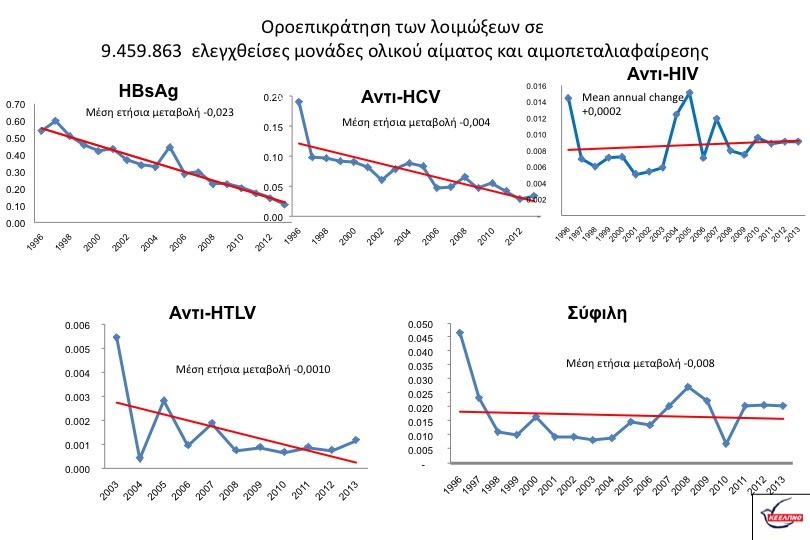
\includegraphics[width=0.7\textwidth]{statistics1.jpg}
	    \caption{Οροεπικράτηση λοιμώξεων σε 9.459.863 ελεγχθείσες μονάδες αίματος και αφαίρεσης αιμοπεταλίων.}
	    \label{fig:statistics1}
\end{figure}	
\begin{figure}[h]
	    \centering
	    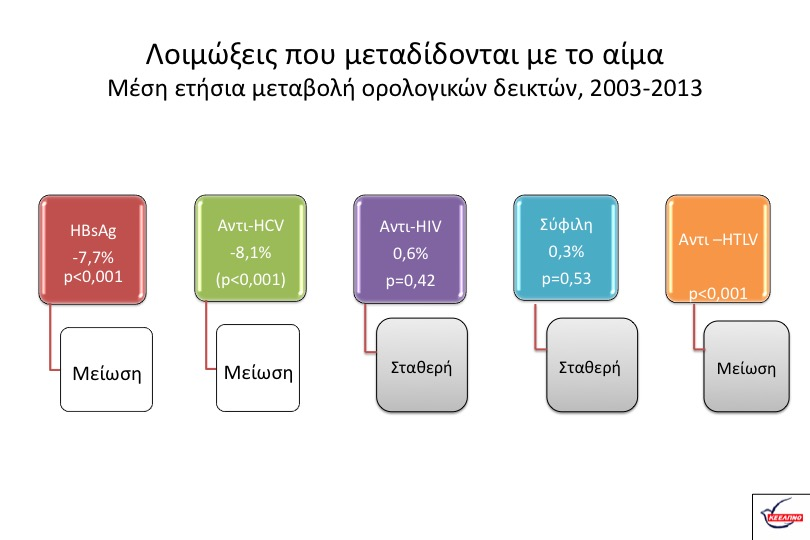
\includegraphics[width=0.7\textwidth]{statistics2.jpg}
	    \caption{Μέση μεταβολή των ορολογικών δεικτών των λοιμώξεων που μεταδίδονται με το αίμα.}
	    \label{fig:statistics2}
\end{figure}	
	Η κατανομή και η ανάλυση των ανεπιθύμητων αντιδράσεων σχετικά με τη μετάγγιση ασθενών το έτος 2013 φαίνονται στο \ref{fig:statistics3}. Το έτος 2013 δηλώθηκαν, μελετήθηκαν και παρουσιάσθηκαν 1092 ανεπιθύμητες αντιδράσεις κατά τη μετάγγιση 729456 προϊόντων αίματος. Η συχνότητα των σοβαρών αντιδράσεων κατά τη μετάγγιση είναι 1/9994 προϊόντα. Κατά τα έτη 1997-2013, δηλώθηκαν επτά θάνατοι, με μεταγγίσεις 8972722 προϊόντων αίματος, συχνότητα 1/281817 προϊόντα με κύρια αίτια: ΑΒΟ ασυμβατότητα, TRALI, βακτηριακή επιμόλυνση.
\begin{figure}[h]
	    \centering
	    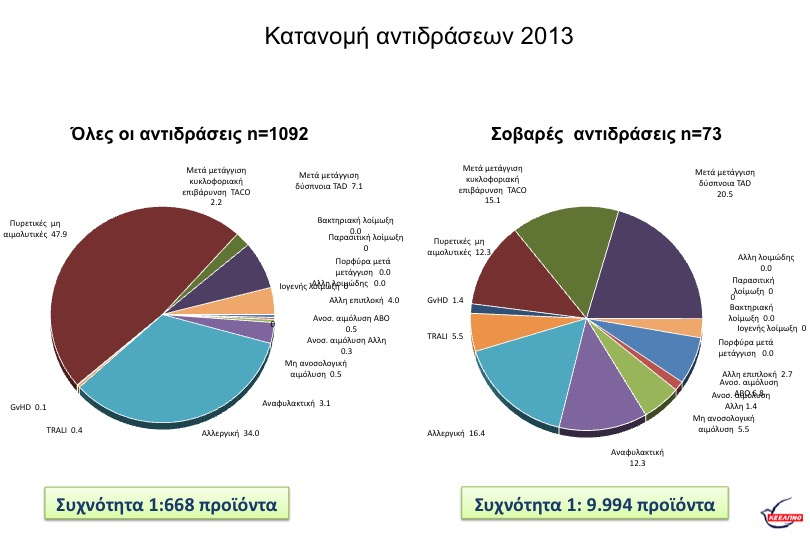
\includegraphics[width=0.7\textwidth]{statistics3.jpg}
	    \caption{Κατανομή αντιδράσεων.}
	    \label{fig:statistics3}
\end{figure}
Στο σχήμα \ref{fig:statistics4} παρουσιάζονται διαγραμματικά οι ανεπιθύμητες αντιδράσεις σχετικές  με την αιμοδοσία. Πιο συγκεκριμένα δηλώθηκαν 148 ανεπιθύμητες αντιδράσεις που αφορούσαν σε σύνολο μεταγγίσεων 44611 μονάδων ερυθρών αιμοσφαιρίων. Καταγράφηκαν (σε ποσοστά επί τοις εκατό) 0.22 πυρετικές, 0.13 αλλεργικές, 0.13 αλλοανοσοποίηση και 0.6 άλλης αιτιολογίας αντίδρασης. Τέλος, στο σχήμα \ref{fig:statistics5} παρουσιάζεται ποσοστιαία ο αριθμός των συμβάντων που έλαβαν χώρα πριν και κατά τη διάρκεια της αιμοδοσίας.
\begin{figure}[h]
	    \centering
	    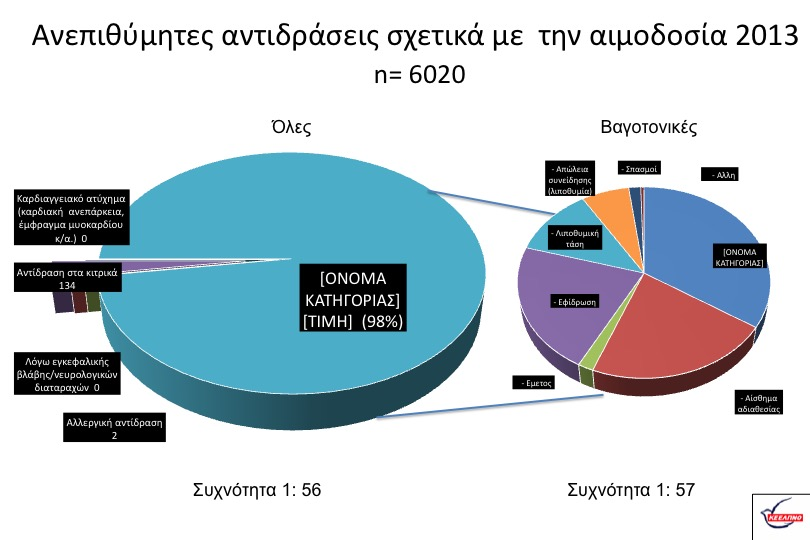
\includegraphics[width=0.7\textwidth]{statistics4.jpg}
	    \caption{Ανεπιθύμητες αντιδράσεις σχετικά με την αιμοδοσία 2013.}
	    \label{fig:statistics4}
\end{figure}
\begin{figure}[h]
	    \centering
	    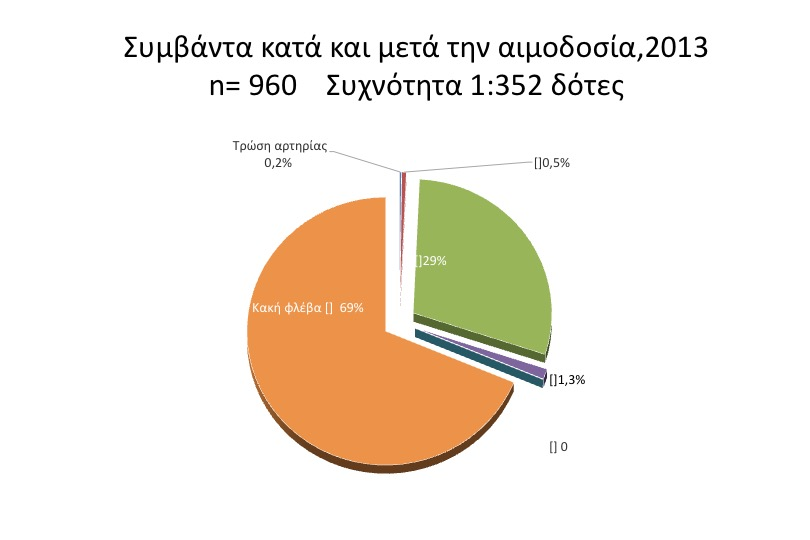
\includegraphics[width=0.7\textwidth]{statistics5.jpg}
	    \caption{ Συμβάντα κατά και μετά την αιμοδοσία, 2013.}
	    \label{fig:statistics5}
\end{figure}
